\documentclass[a4paper, 12pt]{article}

\usepackage[en-GB]{datetime2}

\usepackage[british]{babel}

\usepackage{subcaption}

\usepackage{graphicx}
\graphicspath{ {./images/} }

\usepackage{svg}
\svgpath{ {./images/} }

% Warning: csquotes should be loaded after fvextra, to avoid a warning from the lineno package.
% Solution: The fvextra package is loaded by minted, so minted should be loaded before csquotes.
% \usepackage[outputdir=./.build/]{minted}
\usepackage{minted}

\usepackage{enumitem}

\usepackage{tabularray}

% https://tex.stackexchange.com/questions/229355/algorithm-algorithmic-algorithmicx-algorithm2e-algpseudocode-confused
\usepackage[beginLComment=\#~, endLComment=~]{algpseudocodex}
\usepackage{algorithm}  % https://ctan.org/pkg/algorithms

\usepackage{csquotes}
\usepackage[style=ieee]{biblatex}
\addbibresource{references.bib}

\usepackage{appendix}

%\usepackage[showframe]{geometry}  % The option showframe is used for debugging overfull \hbox or \vbox
\usepackage{geometry}
% Left margin: 1.25 inches (32 mm) recommended for binding; 1 inch minimum.
% Right, top, and bottom margin: 1 inch recommended; 0.75 inches (19 mm) minimum
\geometry{left=1in, right=1in, top=1in, bottom=1in}

\usepackage{setspace}
\setlength{\parskip}{10pt plus 4pt minus 2pt}  % sets spacing between paragraphs

% https://overleaf.com/learn/latex/Questions/I_have_a_custom_font_I%27d_like_to_load_to_my_document._How_can_I_do_this%3F
% Check that all fonts are embedded: pdffonts .\.build\main.pdf
% Pay attention to ISO-31 compliant(ish)

\usepackage[otfmath]{XCharter}  % loads fontspec, unicode-math, and sets XCharter-Math.otf
% \setmathfont{latinmodern-math.otf}[range=cal]  % Latin Modern Math is a clone of Knuth’s Computer Modern but \mathcal alphabet is based on Euler Calligraphic.
% https://tex.stackexchange.com/questions/504856/why-does-setmathfonttex-gyre-bonum-math-not-work
\setmathfont{texgyredejavu-math.otf}[range=cal]

% \usepackage{amsmath}
% \usepackage{unicode-math}
% \setmainfont[
%   UprightFont = *,
%   ItalicFont = *-Italic,
%   BoldFont = *-Demi,
%   BoldItalicFont = *-DemiItalic,
%   Extension = .otf
% ]{LucidaBrightOT}
% \setmathfont{LucidaBrightMathOT}
% \setmathfont[version=bold]{LucidaBrightMathOT-Demi}

\DeclareMathAlphabet{\mathpzc}{OT1}{pzc}{m}{it}


\usepackage{hyperref}  % Loading hyperref last: very few packages should come later than this one
\hypersetup{
   colorlinks = true,  % to avoid the borders around hyperlinks
   citecolor  = black,
   filecolor  = black,
   linkcolor  = black,
   urlcolor   = black,
}

\begin{document}
\begin{frame}[fragile]\centering

\begin{columns}[T]



%%%% First Column
\begin{column}{.46\textwidth}

\begin{block}{Apotheoses and Momentousness}
\begin{itemize}
\item \textbf{AlphaGo} $\rightarrow$ AlphaGo Zero $\rightarrow$ AlphaZero $\rightarrow$ MuZero
\item \textbf{ChatGPT} fine-tuned in a process called \emph{reinforcement learning from human feedback}
\item Ability to tackle problems that are too complicated to model accurately with traditional approaches
\end{itemize}
\end{block}

\begin{block}{Aspirations}
\begin{itemize}
\item \textbf{Implement} SOTA DRL algorithms
\item \textbf{Implement} training environments in a simulator
\item \textbf{Train} policies and \textbf{evaluate} them
\end{itemize}
\end{block}

\begin{block}{Attainments}
\begin{itemize}
\item \textbf{Implemented} a library and a simulation environment
\item Large amount of \textbf{experiments} were conducted
\item \textbf{Trained} polices in a small empty indoor environment
\item Developed \textbf{skills} and \textbf{insights} on DRL and AI
\end{itemize}
\end{block}

\begin{block}{Design for the DRL Library}
\begin{itemize}
\item \textbf{Modular} and \textbf{composable}
\begin{figure}[htbp]
\centering
\includesvg[inkscapelatex=false,pretex=\fontsize{9}{12}\selectfont,width=0.9\textwidth]{SAC}
\caption{UML class diagram of the Soft Actor-Critic algorithm}
\end{figure}
\item \textbf{Unit-tested} with \emph{pytest} and \textbf{integration-tested} on various \emph{Gymnasium's} built-in environments
\item \textbf{Packaged} with the latest PyPA specification
\end{itemize}
\end{block}

\begin{block}{Soft Actor-Critic}
\begin{scriptsize}
\begin{algorithmic}
\State Optimal policy $\pi\mbox{*} = \operatorname*{\mathrm{arg\,max}}_\pi \sum_t \mathop{\mathbb{E}}_{(s_t,a_t)\sim\rho_\pi}\left[r(s_t,a_t)+\alpha\mathcal{H}(\pi(\cdot|s_t))\right]$
\State Initialise critic networks $Q_{\theta_1}$, $Q_{\theta_2}$, and actor network $\pi_\phi$ with random parameters $\theta_1$, $\theta_2$, $\phi$
\State Initialise target network weights $\overline{\theta}_i \gets \theta_i$  for $i \in \left\{1,2\right\}$
\State Initialise an empty replay buffer $\mathcal{B}$
\For{each iteration}
    \For{each environment step}
        \State $a_t \sim \pi_\phi(\cdot|s_t)$
        \State $s_{t+1} \sim p(\cdot|s_t,a_t)$
        \State $\mathcal{B} \gets \mathcal{B} \cup \left\{(s_t,a_t,r(s_t,a_t),s_{t+1})\right\}$
    \EndFor
    \For{each gradient step}
        \State $\theta_i \gets \theta_i - \lambda_Q\hat\nabla_{\theta_i}J_Q(\theta_i)$ for $i \in \left\{1,2\right\}$
        \State $\phi \gets \phi - \lambda_\pi\hat\nabla_{\phi}J_\pi(\phi)$
        \State $\alpha \gets \alpha - \lambda\hat\nabla_{\alpha}J(\alpha)$
        \State $\overline{\theta}_i \gets \tau\theta_i + (1-\tau)\overline{\theta}_i$ for $i \in \left\{1,2\right\}$
    \EndFor
\EndFor
\State where $\hat\nabla J$ denotes the estimated gradient of an objective function, $\overline{\theta}$ denotes an exponentially moving average of $\theta$, $\lambda$ denotes the learning rate, and $\alpha$ is the temperature parameter that determines the relative importance of the entropy term versus the reward.
\end{algorithmic}
\end{scriptsize}
\end{block}

\end{column}



%%%% Second Column
\begin{column}{.46\textwidth}

\begin{block}{Design for the Training Environment}
\begin{figure}[htbp]
\centering
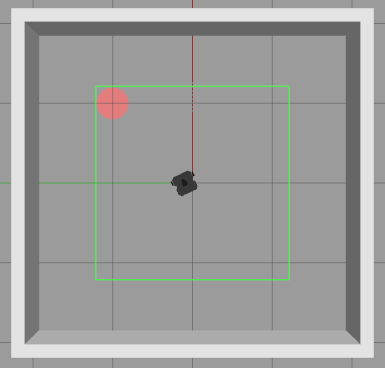
\includegraphics[width=0.32\textwidth]{gazebo.png}
\caption{Aerial view of the venue in Gazebo Classic}
\end{figure}
\begin{itemize}
\item Observed state space:
\begin{equation*}
    \mathcal{S} = (x, d),
\end{equation*}
where $x$ is the data from LiDAR, and $d$ is the relative distance of the navigation goal w.r.t the robot.
\item Action space:
\begin{equation*}
    \mathcal{A} = (v, \omega),
\end{equation*}
where $v$ and $\omega$ are respectively the linear and angular velocity of the robot.
\item Reward shaping
\begin{equation*}
    \mathcal{R}(s_t, a_t) = \begin{cases}
    \mathcal{R}_\text{goal}, &\text{if $d_t < d_\text{th}$}\\
    \mathcal{R}_\text{obstacle}, &\text{if $x_t < x_\text{th}$}\\
    c (d_t - d_{t-1}), &\text{otherwise.}
    \end{cases}
\end{equation*}
Notice that $c$ is an amplification factor and a parameter of the environment, $s_t\in\mathcal{S}$, and $a_t\in\mathcal{A}$.
\end{itemize}
\end{block}

\begin{block}{Limitations of Contemporary DRL}
\begin{itemize}
\item \textbf{Partial} observability
\item \textbf{Sparse} rewards
\item Catastrophic forgetting
    \begin{figure}[htbp]
    \centering
    \includesvg[pretex=\tiny,width=0.59\textwidth]{InvertedDoublePendulum-episodic-return}
    \caption{Episodic return of TD3 on InvertedDoublePendulum}
    \end{figure}
\item Transfer learning
\item Exploration-exploitation trade-off
\end{itemize}
\end{block}

\begin{block}{Conclusions and Future Work}
\begin{itemize}
\item Explored DRL by DIY and experimenting
\item This case study demonstrates benefits and shortcomings of DRL
\item Upgrade to non-stationary env to explore what difference would make on the policies trained
\end{itemize}
\end{block}

\end{column}

\end{columns}



\begin{block}{Selected References}
\begin{tiny}
\begin{itemize}
\item L. Tai, G. Paolo, and M. Liu, "Virtual-to-real deep reinforcement learning: Continuous control of mobile robots for mapless navigation," in \emph{IEEE/RSJ Int. Conf. on Intelligent Robots and Systems (IROS)}. IEEE, 2017, pp. 31-36.
\item T. Haarnoja, A. Zhou, P. Abbeel, and S. Levine, “Soft actor-critic: Off-policy maximum entropy deep reinforcement learning with a stochastic actor,” in \emph{Int. Conf. on Machine Learning}, 2018.
\item P. Henderson, R. Islam, P. Bachman, J. Pineau, D. Precup, and D. Meger, "Deep reinforcement learning that matters," in \emph{AAAI Conf. on Artificial Intelligence}, 2018.
\end{itemize}
\end{tiny}
\end{block}



\end{frame}
\end{document}